\documentclass{article}
\usepackage{icmcsmc2014}
\usepackage{times}
\usepackage{ifpdf}
\usepackage[english]{babel}
%\usepackage{cite}
\usepackage{fancyvrb}
\usepackage[autostyle]{csquotes}  
%%%%%%%%%%%%%%%%%%%%%%%% Some useful packages %%%%%%%%%%%%%%%%%%%%%%%%%%%%%%%
%%%%%%%%%%%%%%%%%%%%%%%% See related documentation %%%%%%%%%%%%%%%%%%%%%%%%%%
%\usepackage{amsmath} % popular packages from Am. Math. Soc. Please use the 
%\usepackage{amssymb} % related math environments (split, subequation, cases,
%\usepackage{amsfonts}% multline, etc.)
%\usepackage{bm}      % Bold Math package, defines the command \bf{}
%\usepackage{paralist}% extended list environments
%%subfig.sty is the modern replacement for subfigure.sty. However, subfig.sty 
%%requires and automatically loads caption.sty which overrides class handling 
%%of captions. To prevent this problem, preload caption.sty with caption=false 
%\usepackage[caption=false]{caption}
%\usepackage[font=footnotesize]{subfig}


%user defined variables
\def\papertitle{Modality Workshop}
\def\firstauthor{First author}
\def\secondauthor{Second author}
\def\thirdauthor{Third author}


% authors so far:
% Till, Miguel

% adds the automatic
% Saves a lot of ouptut space in PDF... after conversion with the distiller
% Delete if you cannot get PS fonts working on your system.

% pdf-tex settings: detect automatically if run by latex or pdflatex
\newif\ifpdf
\ifx\pdfoutput\relax
\else
   \ifcase\pdfoutput
      \pdffalse
   \else
      \pdftrue
\fi

\ifpdf % compiling with pdflatex
  \usepackage[pdftex,
    pdftitle={\papertitle},
    pdfauthor={\firstauthor, \secondauthor, \thirdauthor},
    bookmarksnumbered, % use section numbers with bookmarks
    pdfstartview=XYZ % start with zoom=100% instead of full screen; 
                     % especially useful if working with a big screen :-)
   ]{hyperref}
  %\pdfcompresslevel=9

  \usepackage[pdftex]{graphicx}
  % declare the path(s) where your graphic files are and their extensions so 
  %you won't have to specify these with every instance of \includegraphics
  \graphicspath{{./figures/}}
  \DeclareGraphicsExtensions{.pdf,.jpeg,.png}

  \usepackage[figure,table]{hypcap}
\fi

%setup the hyperref package - make the links black without a surrounding frame
\hypersetup{
    colorlinks,%
    citecolor=black,%
    filecolor=black,%
    linkcolor=black,%
    urlcolor=black
}


% Title.
% ------
\title{\papertitle}

% Authors
% Please note that submissions are NOT anonymous, therefore 
% authors' names have to be VISIBLE in your manuscript. 
%
% Single address
% To use with only one author or several with the same address
% ---------------
%\oneauthor
%   {\firstauthor} {Affiliation1 \\ %
%     {\tt \href{mailto:author1@smcnetwork.org}{author1@smcnetwork.org}}}

%Two addresses
%--------------
% \twoauthors
%   {\firstauthor} {Affiliation1 \\ %
%     {\tt \href{mailto:author1@smcnetwork.org}{author1@smcnetwork.org}}}
%   {\secondauthor} {Affiliation2 \\ %
%     {\tt \href{mailto:author2@smcnetwork.org}{author2@smcnetwork.org}}}

% Three addresses
% --------------
 \threeauthors
   {\firstauthor} {Affiliation1 \\ %
     {\tt \href{mailto:author1@smcnetwork.org}{author1@smcnetwork.org}}}
   {\secondauthor} {Affiliation2 \\ %
     {\tt \href{mailto:author2@smcnetwork.org}{author2@smcnetwork.org}}}
   {\thirdauthor} { Affiliation3 \\ %
     {\tt \href{mailto:author3@smcnetwork.org}{author3@smcnetwork.org}}}

\newcommand{\todo}[1] {\emph{\textbf{TODO:} #1}}
\DefineShortVerb{\|}


\begin{document}
%
\capstartfalse
\maketitle
\capstarttrue
%
\begin{abstract}
The Modality Toolkit aims to improve and facilitate the use of digital technology within interactive sound art and music. 
Written in SuperCollider, it simplifies the creation of individual electronic instruments by combining custom sound engines with off-the-shelf controllers. 
To this end, a common code interface, |MKtl|, is used to connect controllers from various sources and protocols. 
Currently, HID and MIDI are supported; GUI-based interfaces can be created on the fly from interface descriptions.

In the workshop, the toolkit is introduced and used by participants to lay out their control ideas and play music with each other.
\end{abstract}

\begin{figure}[h]
	\centering
		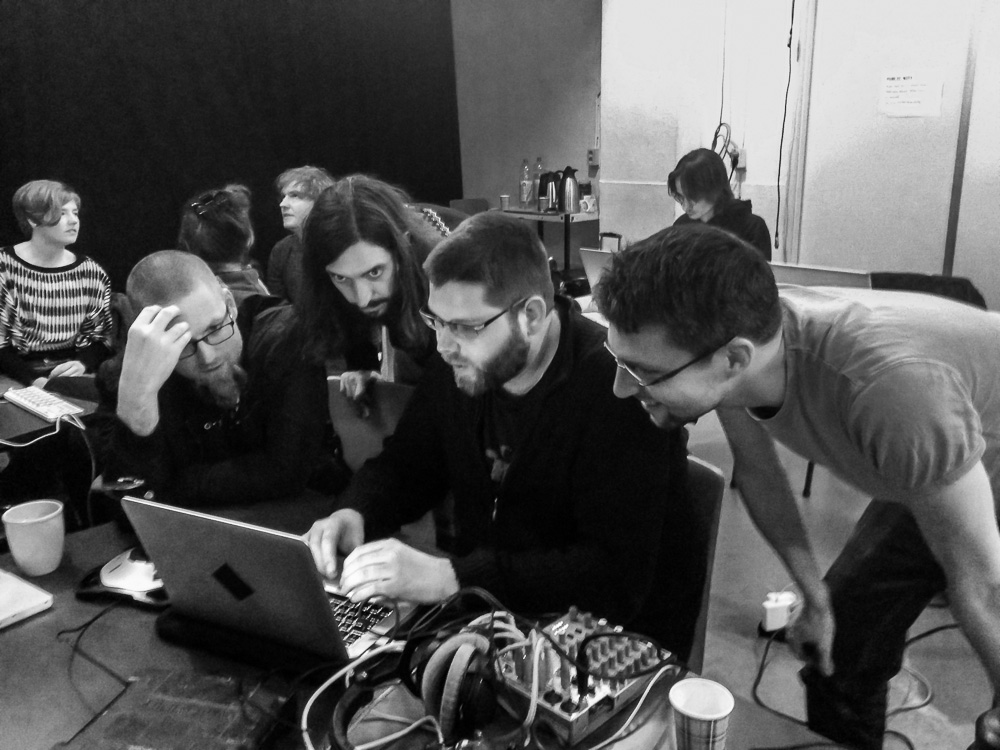
\includegraphics[width=\columnwidth]{../media/20140403-IMG_1667.jpg}
	\caption{A participant gets help by members of the ModalityTeam at a public workshop at STEIM in April 2014.}
	\label{fig:media_20140331-IMG_5976}
\end{figure}




\section{Introduction}
\label{sec:introduction}

The proposed workshop accompanies the paper ``Advances in Modality''.

The name \emph{Modality} arose from the idea to investigate the creation and extensive use of modal interfaces.
One particular strength of such modal interfaces is that they allow fast changes and therefore a broader variety for sonic discovery.
This can be of benefit when, for example, improvising with musicians playing acoustic instruments.
Out of this arouse the question on how HCI interfaces can be both conceptualised and actually built, in which a small set of physical controls are used for numerous purposes.
We contend that integration of such on-the-fly remapping features helps to create flexible instruments that are powerful yet interesting and therefore rewarding to play and listen to. 


\section{Workshop content}
\label{sec:workshop_content}

The concept of the workshop is to be as “hands-­on” as possible.
Participants will learn how to use the Modality toolkit, create their own instruments, and play together with their creations. 
Under the guidance of the Modality Work Group, each participant will be able to work on his or her own instrument, and use and play it along with the other participants.

In detail, the outline of the workshop is as follows:

\begin{enumerate}\itemsep0em
	\item brief introduction to the Modality toolkit,
	\item an installation party, in which the toolkit is installed (takes 5-10 minutes),
	\item mapping out devices (i.e., writing description files for them), in case the devices brought are not yet specified in Modality (contributing to the library of known devices),
	\item accessing devices and using data from devices,
	\item creating a basic sound--controller setup,
	\item first show-and-tell, performing with the system
	\item working out event logic with the goal to create meaningful and interesting relationships between controller data and audio processes,
	\item swap controllers and share sounds between participants,
	\item adaption of the setup and manipulation of data streams,
	\item performing with the system
\end{enumerate}


\section{Intended audience and hardware to bring}
\label{sec:participants}

Workshop participants should have basic knowledge in programming sounds in SuperCollider, e.g. with |SynthDef| or |Ndef|. 
This can be, however, low-profile; having worked through one of the SuperCollider tutorials on how to make sounds should be enough.

Additionally, each participant is required to bring
\begin{itemize}\itemsep0em
	\item at least one MIDI or HID controller such as a game gad, a joystick or a fader box, 
	\item a laptop with a recent version of SuperCollider installed, 
	\item a mini jack to mono jacks cable to connect the laptop to a mixing desk, and
	\item a pair of headphones.
\end{itemize}

The hosting institution should provide a stereo pair of speakers including amplification and a mixing desk.


\section{Workshop leaders}
\label{sec:workshop_leaders}

The ModalityTeam, an international and transdisciplinary group of people that see themselves as users and developers for SuperCollider, meets at regular intervals to work on the library, discuss issues around music performance and composition, and perform in self-organised concerts.

The Modality team is (in alphabetical order):
    Marije Baalman,
    Tim Blechmann,
    Till Bovermann,
    Alberto de Campo,
    Jeff Carey,
    Bj\o{}rnar Habbestad,
    Dominik Hildebrand Marques Lopes,
    Amelie Hinrichsen,
    Robert van Heumen,
    Hannes Hoelzl,
    Miguel Negr\~{a}o, and
    Wouter Snoei.

The workshop will be lead by at least two members of the ModalityTeam.


\begin{acknowledgments}
Associated organisations are (in alphabetical order):
BEK,
the project \emph{Design, Development and Dissemination of New Musical Instruments} of UdK Berlin/TU Berlin, supported by the Einstein Foundation,
nescivi, and
STEIM.

The Modality meetings have been funded by Bergen Kommune, Nordisk Kulturfond and Creative Industries Fund NL.
\end{acknowledgments} 

%%%%%%%%%%%%%%%%%%%%%%%%%%%%%%%%%%%%%%%%%%%%%%%%%%%%%%%%%%%%%%%%%%%%%%%%%%%%%
%bibliography here
\bibliography{smacsmc2014template}

\end{document}
